\documentclass[conference]{IEEEtran}
\IEEEoverridecommandlockouts

\usepackage{cite}
\usepackage{amsmath,amssymb,amsfonts}
\usepackage{graphicx}
\usepackage{textcomp}
\usepackage{xcolor}
\usepackage{booktabs}
\usepackage{multirow}
\usepackage{array}
\usepackage{url}
\usepackage{placeins}
\setlength{\textfloatsep}{6pt plus 1pt minus 2pt}
\setlength{\floatsep}{6pt plus 1pt minus 2pt}
\setlength{\intextsep}{6pt plus 1pt minus 2pt}
\renewcommand{\topfraction}{0.95}
\renewcommand{\dbltopfraction}{0.95}
\renewcommand{\textfraction}{0.05}
\renewcommand{\floatpagefraction}{0.75}
\renewcommand{\dblfloatpagefraction}{0.75}

\def\BibTeX{{\rm B\kern-.05em{\sc i\kern-.025em b}\kern-.08em
    T\kern-.1667em\lower.7ex\hbox{E}\kern-.125emX}}

\begin{document}

\title{ORIGIN-Ax: Origin-Constrained Graph Refinement for Identifiable Latent Axes in Spatial Transcriptomics}

\author{\IEEEauthorblockN{Anonymous Authors}}

\maketitle
\begin{abstract}
Decomposition methods in spatial transcriptomics, such as NMF, ICA, and consensus factorization, convert high-dimensional tumor data into latent axes with gene loadings and spatial activity patterns. Yet in mixed tumor microenvironments, a coherent axis may reflect malignant biology, normal epithelium, stroma, immune infiltration, or unresolved mixtures rather than the intended target source. We present ORIGIN-Ax, a post-decomposition framework that recasts latent-axis interpretation as origin-constrained claim control. Given candidate axes from existing methods, ORIGIN-Ax constructs an origin-aware family graph, grouping axes only when expression loadings and cellular-source evidence are compatible. Families are labeled as target-supported, off-target, or non-identifiable using loading-weighted target evidence, off-target/decoy evidence, family consensus, held-out audits, and optional anchors. Across controlled benchmarks, pseudo-spatial mixtures, Xenium melanoma, target-swap controls, and a Visium HD colorectal cancer stress test, ORIGIN-Ax preserves recoverable target signals while reducing unsupported target-like promotions under predefined claim-risk audits. ORIGIN-Ax provides an auditable interpretation layer for gene-loading axes in complex spatial tissues.
\end{abstract}

\begin{IEEEkeywords}
spatial transcriptomics, latent-axis interpretation, gene programs, origin-constrained graph, claim control, tumor microenvironment
\end{IEEEkeywords}

\section{Introduction}

Spatial transcriptomics measures gene expression while preserving tissue location, enabling detailed studies of tumor architecture, immune infiltration, stromal remodeling, and spatially localized cell states~\cite{stahl2016visualization,tian2023expanding}. To summarize these high-dimensional measurements, many analyses apply decomposition methods such as non-negative matrix factorization (NMF), independent component analysis (ICA), or consensus factorization to extract latent expression programs~\cite{lee1999learning,hyvarinen2000ica,kotliar2019cnmf}. In this work, a \emph{latent axis} denotes a weighted gene program together with a spatial activity score across tissue locations.

However, the biological origin of such an axis is often ambiguous in tumor tissue. A spatially coherent factor enriched for plausible marker genes may not originate from the intended target cell population. Because malignant cells, normal epithelium, immune cells, stromal cells, and mixed boundary regions frequently occupy nearby spatial neighborhoods, a continuous expression axis may reflect target biology, off-target tissue structure, technical effects, or unresolved mixtures. The central difficulty is therefore not simply naming an axis, but determining whether a specific origin claim is sufficiently justified by the available evidence.

Existing evidence sources help but do not fully resolve this axis-level claim problem. Top genes, marker scores, and pathway enrichment describe program content~\cite{subramanian2005gsea,zhang2019cellmarker}; spatial maps show activity patterns; deconvolution estimates local cell-type composition~\cite{kleshchevnikov2022cell2location,cable2022rctd}; and orthogonal signals such as CNV inference, histology, or protein markers provide additional context. Nevertheless, these signals are rarely organized into a formal, transparent decision rule for whether a continuous gene-loading axis should be accepted as target-origin, rejected as off-target, or reported as non-identifiable. This gap often leads to subjective and difficult-to-audit interpretations across datasets and target definitions.

We formulate latent-axis interpretation as \emph{origin-constrained claim control}. Under this perspective, the key question is whether the evidence sufficiently supports the claim that an axis originates from a user-defined target source (e.g., malignant cells, myeloid inflammation, or stromal remodeling). A target claim should be promoted only when target evidence outweighs plausible competing origins; conversely, an axis should be rejected or labeled non-identifiable when normal epithelial, stromal, immune, endothelial, or technical decoy evidence provides a better explanation.

We introduce ORIGIN-Ax, a post-decomposition interpretation layer for gene-loading latent axes. ORIGIN-Ax does not replace upstream factorization methods but audits biological claims before downstream analysis. Given candidate axes, it constructs an origin-aware family graph whose edges depend on both expression similarity and origin evidence. Axes are grouped only when their loading patterns and source evidence are compatible, while seemingly similar axes better explained by different origins are deliberately separated. Thus, origin evidence actively shapes family structure rather than serving merely as a post-hoc score.

Each family receives a conservative label---target-supported, off-target, or non-identifiable---based on loading-weighted target evidence, off-target/decoy evidence, family consensus, held-out target-gene audits, and optional orthogonal anchors. Our contributions are threefold: (1) we recast latent-axis interpretation from marker-based annotation into origin-constrained claim control; (2) we introduce an origin-aware axis-family graph for evidence-driven grouping; and (3) we demonstrate, across controlled benchmarks, pseudo-spatial mixtures, real tumor datasets (Xenium melanoma and Visium HD colorectal cancer), and target-swap controls, that ORIGIN-Ax preserves recoverable target signals while reducing unsupported target-like promotions under predefined audit rules rather than estimating absolute biological false-positive rates.

\section{Related Work}

\subsection{Latent Decomposition and Gene Program Discovery}

NMF, ICA, and related factorization methods extract low-dimensional structure
from high-dimensional expression data~\cite{lee1999learning,hyvarinen2000ica}.
In single-cell and spatial transcriptomics, repeated or consensus-like
factorization and spatial co-expression methods identify gene programs,
spatial factors, and activity gradients~\cite{kotliar2019cnmf,higgins2025stihc}.
Spatial embedding and domain-detection methods similarly provide useful
representations, but address upstream pattern discovery rather than
target-origin claim validation. ORIGIN-Ax is therefore evaluated as an
interpretation-control layer over candidate axes, not as a replacement for
embedding, clustering, or domain-detection models.

\subsection{Annotation, Deconvolution, and External Evidence}

Standard interpretation tools include top-gene inspection, marker scoring,
pathway enrichment, and curated marker resources~\cite{subramanian2005gsea,zhang2019cellmarker}.
Spatial deconvolution estimates cell-type abundance in spots or
neighborhoods~\cite{kleshchevnikov2022cell2location,cable2022rctd}, and recent
spatial genomics discussions emphasize methods that connect spatial
measurements to explicit biological questions~\cite{jena2024openquestions}.
These evidence sources are useful, but they do not by themselves provide a
reproducible rule for whether a continuous gene-loading axis should be
interpreted as target-origin rather than off-target or mixed-origin signal.

\subsection{Origin-Aware Claim Control}

Most workflows ask whether a factor is stable, spatially coherent,
marker-enriched, or correlated with external covariates. ORIGIN-Ax instead
models competing origin evidence and performs interpretation at the family
level. A coherent family can be rejected when normal epithelial, stromal,
immune, endothelial, or technical evidence better explains the axis than the
target source. This distinguishes ORIGIN-Ax from expression-only clustering
followed by post-hoc annotation, because origin evidence actively shapes the
graph on which interpretable families are defined.

\section{Problem Formulation}

Let an upstream decomposition method, such as ICA, NMF, or
repeated NMF, produce a set of candidate latent axes
$\mathcal{A}=\{a_i\}_{i=1}^{m}$ from a spatial transcriptomic
expression matrix. Each axis $a_i=(\ell_i,z_i)$ contains a gene
loading vector $\ell_i$ and a spatial or neighborhood-level score
vector $z_i$. ORIGIN-Ax does not relearn the factorization of the
expression matrix. Instead, it addresses a post-decomposition
interpretation problem: given a user-defined target-origin claim,
determine whether the available evidence supports interpreting
one or more candidate axes as target-origin programs.

Inputs are candidate axes, target evidence, off-target/decoy evidence, and
optional anchors such as cell-type labels, CNV-like latents, histology, or
spatial niche summaries. Held-out target genes are reserved for audit rather
than primary scoring. The output is a set of refined axis families
$\mathcal{F}=\{F_k\}$ with labels:
\[
\begin{aligned}
y(F_k)\in\{&
\texttt{target\_axis},\texttt{off\_target},\\
&\texttt{non\_identifiable}\}.
\end{aligned}
\]
A separate output flag \texttt{not\_target\_axis} is used only to exclude
families from target-origin downstream analyses; it is not a fourth semantic
category.

The goal is not to name every axis, but to decide whether a specific
target-origin claim is sufficiently supported relative to competing origins. A
family is promoted only when target evidence dominates, rejected when an
off-target origin better explains it, and marked non-identifiable when evidence
is insufficient for a safe target-origin claim.

\section{Methods}

\begin{figure*}[!t]
\centering
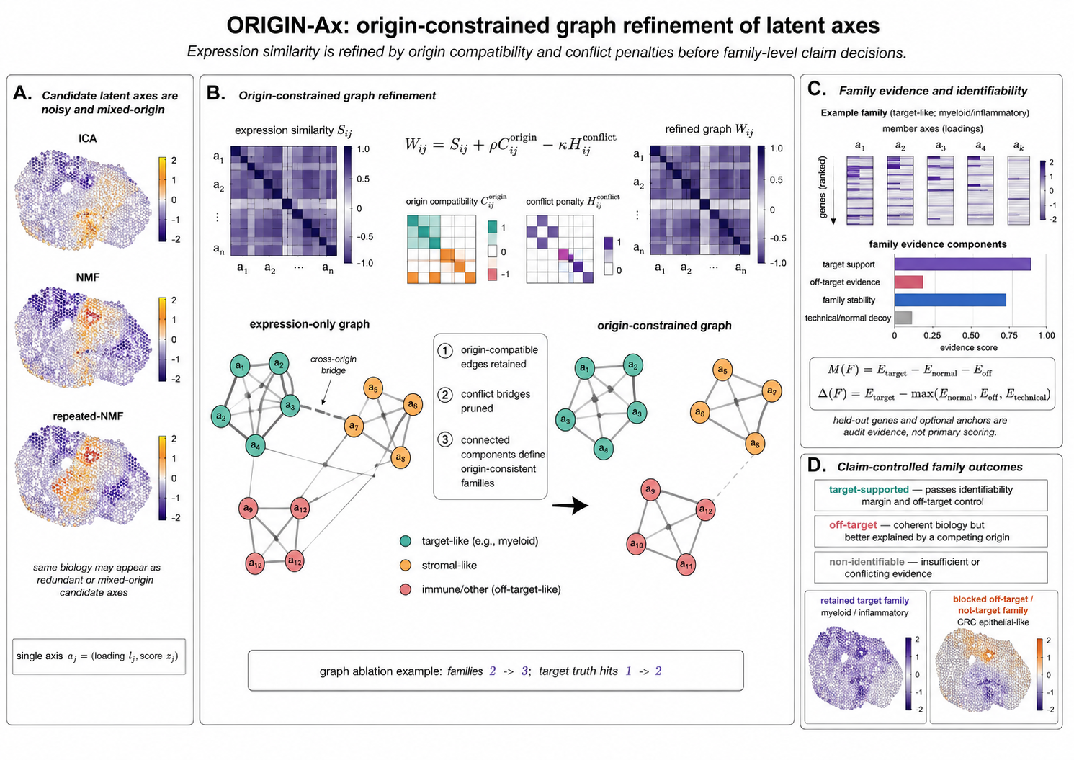
\includegraphics[width=0.94\linewidth]{figures/fig1_workflow.pdf}
\caption{ORIGIN-Ax converts candidate axes into origin profiles, refines them
with compatibility- and conflict-aware graph edges, assembles origin-consistent
families, and assigns target-supported, off-target, or non-identifiable labels.}
\label{fig:workflow}
\end{figure*}

\subsection{Overview}

ORIGIN-Ax is a post-decomposition refinement layer
(Fig.~\ref{fig:workflow}). It computes expression similarity and origin
profiles, builds an origin-constrained graph, forms direction-aligned family
consensus axes, and assigns claim labels using target support, off-target
evidence, stability, held-out audits, and optional anchors.

\subsection{Candidate Axis Interface}

Candidate axes come from raw ICA, raw NMF, high-target subset decompositions, or
repeated-NMF runs. Each provides gene loadings and spatial/neighborhood scores;
ORIGIN-Ax does not re-optimize reconstruction and applies the same graph,
scoring, and labeling rules to all inputs.

\subsection{Origin-Constrained Axis Family Graph}

Candidate axes are grouped before interpretation, but family construction is
not based on expression similarity alone. For axes $a_i$ and $a_j$, ORIGIN-Ax
first computes an expression similarity
\begin{equation}
S(a_i,a_j)=0.6|\mathrm{corr}(\ell_i,\ell_j)|+0.4J(T_i,T_j),
\end{equation}
where $T_i$ is the top-gene set of axis $a_i$ and $J(\cdot,\cdot)$ is Jaccard
similarity. Loading correlation captures global agreement across genes,
whereas top-gene overlap captures whether the interpretable high-loading tail
is shared.

Each axis also receives a competing-origin profile
\begin{equation}
e_i=(E_{\mathrm{target},i},E_{\mathrm{normal},i},
E_{\mathrm{TME},i},E_{\mathrm{tech},i}),
\end{equation}
where each term is computed from loading-tail-weighted gene evidence using
the positive high-loading genes of $a_i$. The dominant origin is the largest
entry of $e_i$, and the axis margin is
\[
\delta_i=E_{\mathrm{target},i}
-\max(E_{\mathrm{normal},i},E_{\mathrm{TME},i},E_{\mathrm{tech},i}).
\]

ORIGIN-Ax then refines the edge weight as
\begin{equation}
W_{ij}=S(a_i,a_j)+\rho C^{\mathrm{origin}}_{ij}
-\kappa H^{\mathrm{conflict}}_{ij},
\end{equation}
where $C^{\mathrm{origin}}_{ij}\in[0,1]$ is the cosine similarity between
origin profiles when the dominant origin agrees and is set to zero otherwise.
$H^{\mathrm{conflict}}_{ij}\in[0,1]$ is set to one for strong cross-origin
bridge edges, including target-dominant versus off-target-dominant pairs with
sufficient evidence. Otherwise, it combines target/off-target co-activation,
margin sign flips, and dominant-origin disagreement.

Origin-compatible axes are therefore kept together, while expression-similar
axes with competing origins are pruned. In our experiments,
$\rho=0.15$, $\kappa=0.60$, and edges are retained when $W_{ij}\geq0.35$.
These fixed defaults avoid post-hoc tuning and implement a transparent rule in
which conflict pruning dominates compatibility reward; sensitivity and ablation
audits assess whether conclusions depend on a single parameter point.

Connected components define axis families. Member loadings are direction-aligned
before averaging into consensus loadings and scores; each family remains
traceable to member axes, source methods, and graph-edge diagnostics.

\subsection{Origin Evidence Vector}

For each gene $g$, a target definition provides target support $u_g$, normal
or target-specific penalty $r_g$, and off-target penalty $o_g$. For a family
$F$, ORIGIN-Ax computes loading-tail-weighted evidence over the positive
high-loading genes:
\begin{equation}
E_{\mathrm{target}}(F)=
\frac{\sum_{g\in P_F}w_{Fg}u_g}
{\sum_{g\in P_F}w_{Fg}+\epsilon},
\end{equation}
\begin{equation}
E_{\mathrm{normal}}(F)=
\frac{\sum_{g\in P_F}w_{Fg}r_g}
{\sum_{g\in P_F}w_{Fg}+\epsilon},
\end{equation}
\begin{equation}
E_{\mathrm{off}}(F)=
\frac{\sum_{g\in P_F}w_{Fg}o_g}
{\sum_{g\in P_F}w_{Fg}+\epsilon}.
\end{equation}
Here $P_F$ is the positive top-loading tail of the consensus axis and $w_{Fg}$
is the positive loading weight. The target-origin margin is
\[
M(F)=E_{\mathrm{target}}(F)-E_{\mathrm{normal}}(F)-E_{\mathrm{off}}(F),
\]
and the identifiability margin is
\begin{equation}
\begin{split}
\Delta(F)=&\,E_{\mathrm{target}}(F)\\
&-\max(E_{\mathrm{normal}}(F),E_{\mathrm{off}}(F),
E_{\mathrm{technical}}(F)).
\end{split}
\end{equation}

Family stability is
\begin{equation}
Q(F)=0.4\min(1,|F|/4)+0.3\min(1,d_F/3)+0.3\bar{s}_F,
\end{equation}
where $|F|$ is member count, $d_F$ is the number of contributing decomposition
sources, and $\bar{s}_F$ is mean within-family loading similarity.

Target and off-target definitions are supplied as binary or confidence-weighted
references rather than learned from the test set. Target support may come from
malignant-only references, high-CNV regions, or curated programs; off-target
references cover normal epithelial, stromal, immune, endothelial, and
tissue-specific false-boundary programs. Anchor genes are removed from
off-target sets in anchor-split experiments, while overlapping non-anchor
markers remain competing evidence. Technical evidence is reserved for supplied
technical references or covariates. CRC gene weights were derived from
CellMarker~\cite{zhang2019cellmarker} and curated false-boundary programs;
Xenium melanoma references were pre-specified marker sets. In target-swap,
stromal/ECM genes become the target and myeloid genes become off-target.

\subsection{Scoring, Auditing, and Labels}

ORIGIN-Ax uses percentile-normalized evidence values:
\begin{equation}
\mathrm{score}(F)=0.6\widetilde{M}(F)+0.4\widetilde{Q}(F)
-\widetilde{E}_{\mathrm{off}}(F).
\end{equation}
Percentile normalization uses the 5th--95th percentile range within each run:
target margin promotes origin support, stability reduces single-axis
overinterpretation, and off-target affinity implements negative evidence.

A family is labeled \texttt{target\_axis} if $\mathrm{score}(F)>0.2$,
$\Delta(F)>0$, and mean family-origin conflict is at most 0.35. It is labeled
\texttt{off\_target} if $\mathrm{score}(F)<-0.2$, $\Delta(F)<-0.05$, or
target-specific off-target evidence dominates; otherwise it is
\texttt{non\_identifiable}. The implementation flag \texttt{not\_target\_axis}
only excludes a family from target-origin downstream analysis.

A target-specific off-target override is triggered when top genes contain at
least two markers from a pre-specified forbidden source. Optional anchors support
attribution checks but cannot rescue failed gene-origin evidence. Positive
experiments split target genes into anchor and held-out subsets; only anchors
score the model, while held-out genes audit strict positives. ORIGIN-Ax is
rule-based because labeled target and false-target axes across tissues and
platforms are not available at sufficient scale.

\subsection{Implementation and Complexity}

All runs use fixed seeds and write candidate tables, graph-edge audits, family
tables, score diagnostics, and final claim summaries. For $m$ candidate axes and
$p$ genes, graph construction costs $O(m^2p)$ and family scoring costs
$O(|F|p)$ per family. In our runs $m=10$--32; at 1000 axes the dense pairwise
matrix is 8.0 MB, although loading comparisons remain quadratic.

\section{Experiments}

\subsection{Datasets and Benchmark Inputs}

We evaluate ORIGIN-Ax in controlled positives with planted target/off-target
blocks, semi-real pseudo-spatial mixtures from Xenium melanoma cells, real
Xenium melanoma neighborhoods with a myeloid/inflammatory target, a
myeloid-to-stromal target-swap control, and a sampled Visium HD CRC stress test
for epithelial overcalling. To test decomposition-agnostic refinement, ORIGIN-Ax
is applied to raw ICA-only, NMF-only, and repeated-NMF consensus-like candidate
axes without regenerating mixed candidates.

\subsection{Evaluation Metrics}

For positives, we report target recovery, held-out target-gene overlap, and, in
real positives, strict positives: target-supported families with held-out
overlap and no forbidden off-target source. For stress tests, we report
unsupported target-like promotions before and after refinement. These are
predefined claim-risk audit events rather than ground-truth false-positive
labels. A candidate is counted as unsupported when it satisfies naive
target-like criteria but lacks held-out support, is dominated by decoy evidence,
or fails the identifiability margin under the specified reference universe. For
CRC, where true malignant-axis labels are unavailable, this means quantifying
malignant-like promotion risk under epithelial-marker, CNV-association, and
high-CNV-presence rules, not claiming absolute biological false positives.

\subsection{Ablation Protocol}

We add fixed ablations using the same candidate axes and family tables: no
family refinement, no off-target penalty, no stability term, and expression-only
versus origin-constrained graph construction. Thresholds are not tuned.

Controlled and pseudo-ST settings serve as development audits. We scan
$\rho\in\{0,0.05,0.10,0.15,0.20,0.30\}$,
$\kappa\in\{0.20,0.40,0.60,0.80,1.00\}$, edge thresholds
$\{0.25,0.30,0.35,0.40,0.45\}$, target/stability weights
$\{0.50/0.50,0.60/0.40,0.70/0.30\}$, and score thresholds
$\{0.10,0.15,0.20,0.25,0.30\}$. A graph tuple is stable if the family count differs
from the selected default by at most one, removes cross-origin bridge edges, and
does not reduce downstream recovery in every development setting; a score tuple
is stable if it retains at least one truth-supported family and produces no
unsupported target call. We also compare marker-only, marker plus off-target
filtering, expression-only graph annotation, and full ORIGIN-Ax interpretation
baselines. To audit split stability, we repeat 50 random anchor/held-out
target-gene splits in the real-positive Xenium setting. We compute empirical
gene-label permutation nulls with 1000 permutations for target margin,
forbidden off-target rejection, and CRC malignant-margin risk, and report
reference-coverage warnings before biological interpretation. Reference warnings
are issued for off-target coverage below 0.30, decoy diversity below 2,
ambiguous-marker fraction above 0.25, or top-gene reference hit rate below 0.15.
To test reference-deletion robustness, we additionally removed 20\%, 40\%, and
60\% of off-target reference genes in the real-positive Xenium setting and
tracked strict-target retention and forbidden off-target rejection; we also
contaminated target references with off-target genes to test whether forbidden
sources remain rejected.
These baselines reflect common interpretation-layer alternatives--top-gene
promotion, negative-reference filtering, and expression-only family annotation--
and test claim control beyond standard post-decomposition practice.

\section{Results}

\subsection{ORIGIN-Ax Retains Target Recovery While Reducing Unsupported Calls}

Across controlled and semi-real positives, ORIGIN-Ax recovered target-origin
families (Fig.~\ref{fig:evidence}). In the controlled positive, it recovered
two target families from 40 candidates and 3 families; balanced and low-purity
pseudo-ST recovered one target family each. In benchmark-refinement mode,
ORIGIN-Ax retained truth-supported pseudo-ST recovery across ICA, NMF, and
repeated-NMF consensus-like inputs while reducing unsupported target-like
promotions under the predefined audit rules (Table~\ref{tab:benchmark}). This
supports the intended role of ORIGIN-Ax as a refinement layer: it reduces
candidate-level overpromotion without replacing upstream decomposition.

\begin{figure}[!t]
\centering
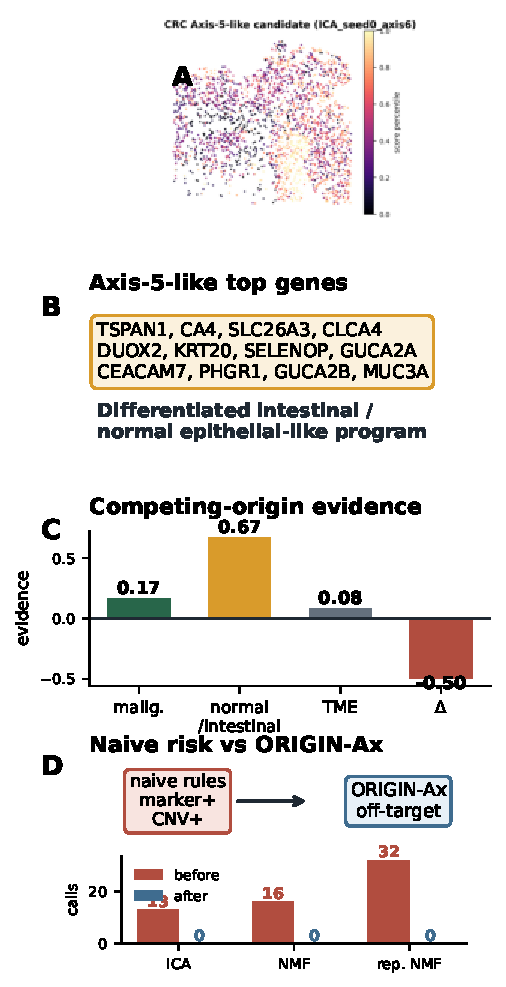
\includegraphics[width=\linewidth]{figures/fig4_crc_axis5_singlecol.pdf}
\caption{CRC epithelial-like stress test. (A) Axis-5-like spatial score map.
(B) Differentiated intestinal / normal epithelial top genes. (C) Normal decoy
evidence gives a negative identifiability margin. (D) ORIGIN-Ax blocks
malignant-like promotion risk across ICA, NMF, and repeated-NMF inputs.}
\label{fig:crc}
\end{figure}

\begin{figure}[!t]
\centering
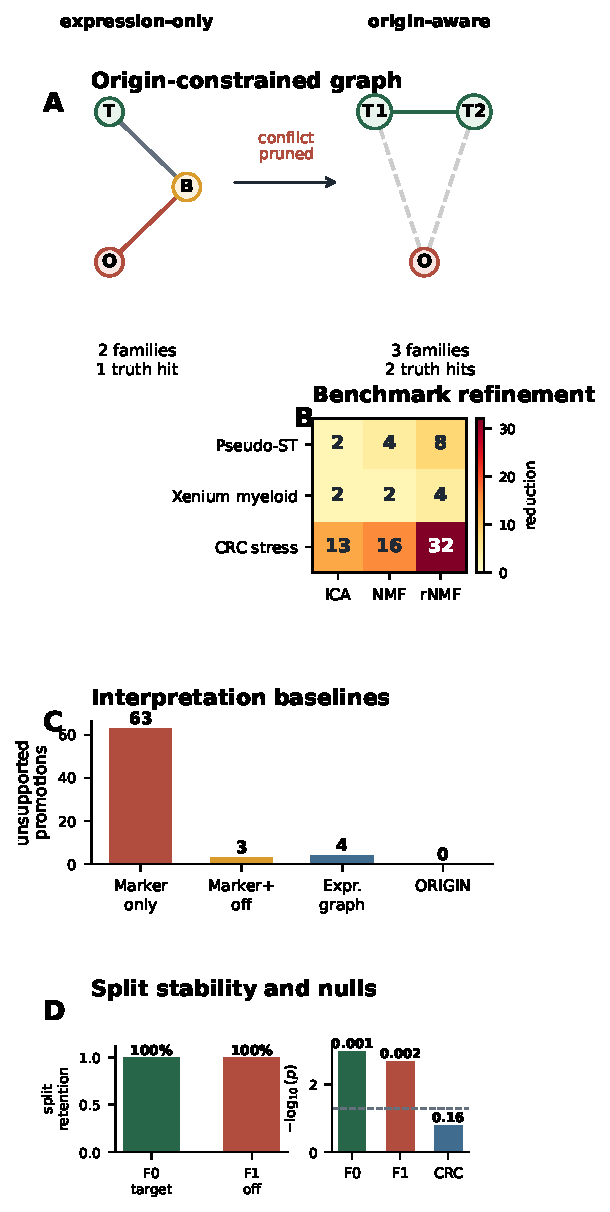
\includegraphics[width=\linewidth]{figures/fig2_evidence_summary_singlecol.pdf}
\caption{Ablation and audit evidence. (A) Origin-constrained graph refinement
changes family construction. (B) Unsupported target-like promotions are reduced
across inputs. (C) Interpretation baselines reduce but do not remove unsupported
promotions. (D) Split-stability and gene-label permutation audits support the
real-positive F0 target, F1 off-target rejection, and non-promotion of the CRC
Axis-5-like malignant claim; the right subpanel uses $-\log_{10}(p)$ bar
heights with empirical $p$ values printed above bars.}
\label{fig:evidence}
\end{figure}

\begin{table*}[t]
\caption{Benchmark-refinement results. ``Before'' counts unsupported
target-like calls from benchmark axes; ``After'' counts unsupported calls after
ORIGIN-Ax refinement. CRC entries are claim-risk audits, not ground-truth
false-positive rates.}
\label{tab:benchmark}
\centering
\scriptsize
\setlength{\tabcolsep}{3pt}
\begin{tabular}{p{0.15\linewidth}p{0.15\linewidth}rrrrrp{0.24\linewidth}}
\toprule
Dataset & Input & Axes & Fam. & Before & After & Target & Conclusion \\
\midrule
Pseudo-ST & raw ICA & 10 & 4 & 2 & 0 & 2 & Truth retained \\
Pseudo-ST & NMF & 10 & 5 & 4 & 0 & 2 & Truth retained \\
Pseudo-ST & rep. NMF & 20 & 5 & 8 & 0 & 2 & Truth retained \\
Xenium & raw ICA & 12 & 3 & 2 & 0 & 0 & Off-target rejected; target absent \\
Xenium & NMF & 12 & 4 & 2 & 0 & 1 & Strict positive; off-target rejected \\
Xenium & rep. NMF & 24 & 4 & 4 & 0 & 1 & Strict positive; off-target rejected \\
CRC & raw ICA & 16 & 6 & 13 & 0 & 0 & Off-target families rejected \\
CRC & NMF & 16 & 5 & 16 & 0 & 0 & Axis-5-like rejected \\
CRC & rep. NMF & 32 & 5 & 32 & 0 & 0 & Axis-5-like rejected \\
\bottomrule
\end{tabular}
\setlength{\tabcolsep}{6pt}
\end{table*}

\begin{table}[!t]
\caption{Interpretation-layer baseline audit aggregated across benchmark rows.}
\label{tab:interpretation_baselines}
\centering
\scriptsize
\setlength{\tabcolsep}{3pt}
\begin{tabular}{p{0.46\linewidth}rrr}
\toprule
Interpretation rule & Target & Unsupported & Truth \\
\midrule
Marker-only top genes & 89 & 63 & 26 \\
Marker plus off-target filter & 29 & 3 & 26 \\
Expression-only graph annotation & 5 & 4 & 1 \\
ORIGIN-Ax full & 8 & 0 & 8 \\
\bottomrule
\end{tabular}
\setlength{\tabcolsep}{6pt}
\end{table}

ORIGIN-Ax reports fewer truth calls because it counts strict family-level claims
rather than every marker-positive candidate, removing duplicate or weak hits.

\begin{table}[!t]
\caption{Compact calibration, baseline, reference, and scaling audits.}
\label{tab:robustness}
\centering
\scriptsize
\setlength{\tabcolsep}{2pt}
\begin{tabular}{p{0.31\linewidth}p{0.63\linewidth}}
\toprule
Audit & Result \\
\midrule
Parameter calibration &
Graph defaults are in the stable plateau: 47/150 tuples stable; score decisions
were robust across all 15 tested tuples on controlled and pseudo-ST settings. \\
Interpretation baselines &
Unsupported promotions: marker-only 63, marker+off-target 3,
expression-only graph 4, ORIGIN-Ax full 0. \\
Reference coverage &
Four target settings triggered no coverage warning; off-target coverage was
0.77--1.00 and decoy diversity was 2--9. \\
Split/null audits and scaling &
F0 target and F1 off-target calls were retained in 50/50 splits; empirical-null
calls matched fixed calls for F0, F1, and CRC Axis-5-like. At 1000 axes, the
pairwise matrix is 8.0 MB but graph construction remains $O(m^2p)$. \\
\bottomrule
\end{tabular}
\setlength{\tabcolsep}{6pt}
\end{table}

\subsection{Real Xenium Melanoma: Target and Off-Target Refinement}

In real Xenium melanoma neighborhoods, ORIGIN-Ax identified F0 as a strict
myeloid/inflammatory target family with held-out target-gene overlap of 4, no
dominant forbidden off-target source, and a significant gene-label null
($p=9.99\times 10^{-4}$). F1 contained melanoma markers
\textit{TYRP1}, \textit{PMEL}, \textit{TYR}, and \textit{MLANA}; ORIGIN-Ax
rejected it as melanoma-like (\texttt{not\_target\_axis}), with null support for
forbidden-source rejection ($p=2.0\times10^{-3}$).

\subsection{Target-Swap Demonstrates Target-Agnostic Refinement}

Using the same Xenium candidate axes, we swapped the target from
myeloid/inflammatory to stromal/fibroblast/ECM. The myeloid-like family was not
a stromal target, whereas the stromal F2-like family was rejected under the
myeloid target but recovered as \texttt{target\_axis} under the stromal target
(Fig.~\ref{fig:swap}).

\begin{figure}[!t]
\centering
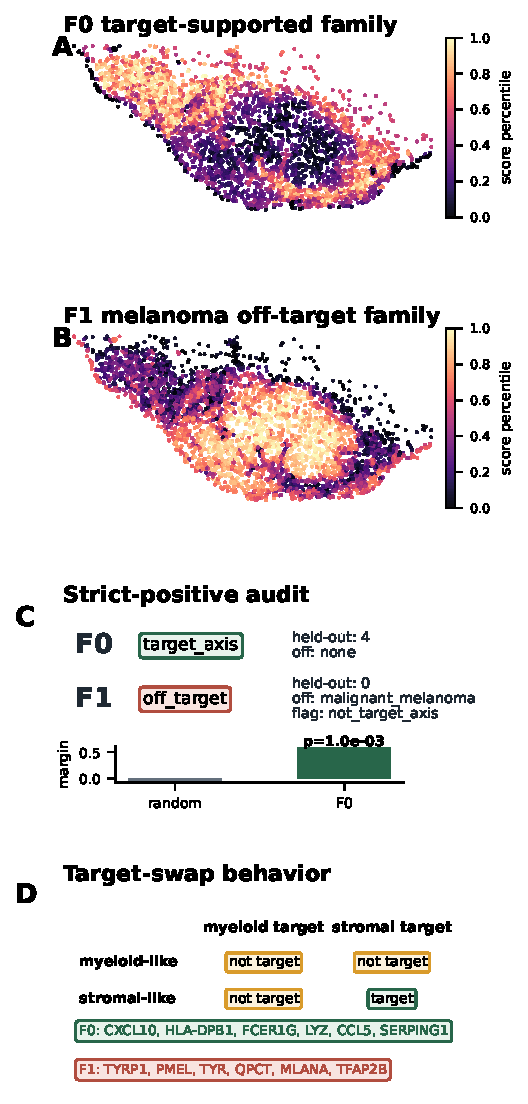
\includegraphics[width=\linewidth]{figures/fig3_target_swap_singlecol.pdf}
\caption{Real Xenium target refinement and target-swap behavior. (A) Myeloid
target family. (B) Melanoma off-target family. (C) Strict-positive and
off-target calls. (D) The same families change calls when the target definition
is swapped.}
\label{fig:swap}
\end{figure}

\subsection{Ablation and Sensitivity Audits}

The controlled positive shows that the origin-constrained graph changes family
construction: target truth hits increase from 1 to 2 without adding false target
calls. Aggregated baselines show 63 unsupported promotions for marker-only, 3
for marker plus off-target filtering, 4 for expression-only graph annotation,
and 0 for full ORIGIN-Ax (Table~\ref{tab:interpretation_baselines}). Additional
audits place defaults in stable plateaus, retain F0/F1 across 50 splits, and
support the Xenium but not CRC Axis-5-like malignant margin
(Table~\ref{tab:robustness}).

\subsection{Visium HD CRC: Blocking Promotion When Decoy Evidence Dominates}

In the Visium HD CRC stress test, an Axis-5-like program contained intestinal
and normal epithelial genes including \textit{TSPAN1}, \textit{CA4},
\textit{SLC26A3}, \textit{CLCA4}, \textit{KRT20}, and \textit{CEACAM7}. Naive
epithelial-marker/CNV rules would call it malignant-like; ORIGIN-Ax labeled it
normal-epithelial/off-target and produced zero CRC target calls across ICA, NMF,
and repeated-NMF inputs.

\section{Discussion and Limitations}

ORIGIN-Ax provides an auditable evidence framework for latent-axis
interpretation: it retains target recovery in positives, reduces unsupported
target-like promotions, rejects a forbidden off-target family, responds to
target-swap definitions, and avoids overcalling a CRC epithelial program as
malignant. In use, researchers run ICA, NMF, repeated-NMF, or another
decomposition, then ORIGIN-Ax produces family tables, strict-positive summaries,
off-target warnings, and claim recommendations. References should be defined
before final calling and include plausible false-boundary programs.

As additional feasibility checks not used for the main claims, ORIGIN-Ax
recovered one strict malignant-breast target family in Xenium breast
neighborhoods (24 candidates, 3 families; top genes included \textit{KRT7},
\textit{EPCAM}, \textit{ERBB2}, \textit{FOXA1}, and \textit{GATA3}) and one
strict lymphoid-immune target family in Xenium lung neighborhoods (24
candidates, 5 families; top genes included \textit{TRAC}, \textit{PTPRC},
\textit{IL7R}, \textit{CD3E}, and \textit{CD3D}). These extra runs used the
unchanged ORIGIN-Ax rules and support feasibility on additional target
definitions, but they do not establish universal parameter optimality.

The anonymous review repository
\url{https://anonymous.4open.science/r/ORIGIN-Ax} includes code, fixed seeds,
reference sets, processed result tables, and figure-generation scripts.

ORIGIN-Ax provides claim control under available evidence rather than solving
all mixture and origin-identification problems. Decisions are conditional on the
reference universe; unknown decoys cannot be rejected and incomplete off-target
references can yield apparent target calls. It does not decontaminate
expression, prove cell-of-origin or clone/niche causality, or replace wet-lab
validation. Real-data experiments lack independent gold standards for every
latent axis, so they audit claim support rather than absolute biological
classification accuracy. ORIGIN-Ax also cannot recover a target program absent
from upstream candidates; non-identifiable is therefore a valid output.

\section{Conclusion}

ORIGIN-Ax is a decomposition-agnostic origin-constrained graph refinement
framework for latent axes in complex spatial transcriptomics data. By combining
expression similarity, origin compatibility, off-target conflict, axis-family
consensus, and non-identifiability labels, it turns candidate gene programs into
auditable target-origin claims. In our audits, this preserves supported target
families, rejects off-target families, and clarifies when an attractive axis
should remain non-identifiable. The framework does not replace upstream
decomposition or prove cell-of-origin, but it provides a practical layer for
preserving supported axes while blocking unsupported biological overpromotion.

\FloatBarrier
\section*{Acknowledgment}

Omitted for anonymous review.

\bibliographystyle{IEEEtran}
\bibliography{references}

\end{document}
